\subsubsection{UC15 - Modifica funzione }
\begin{figure}[H]
	\centering
	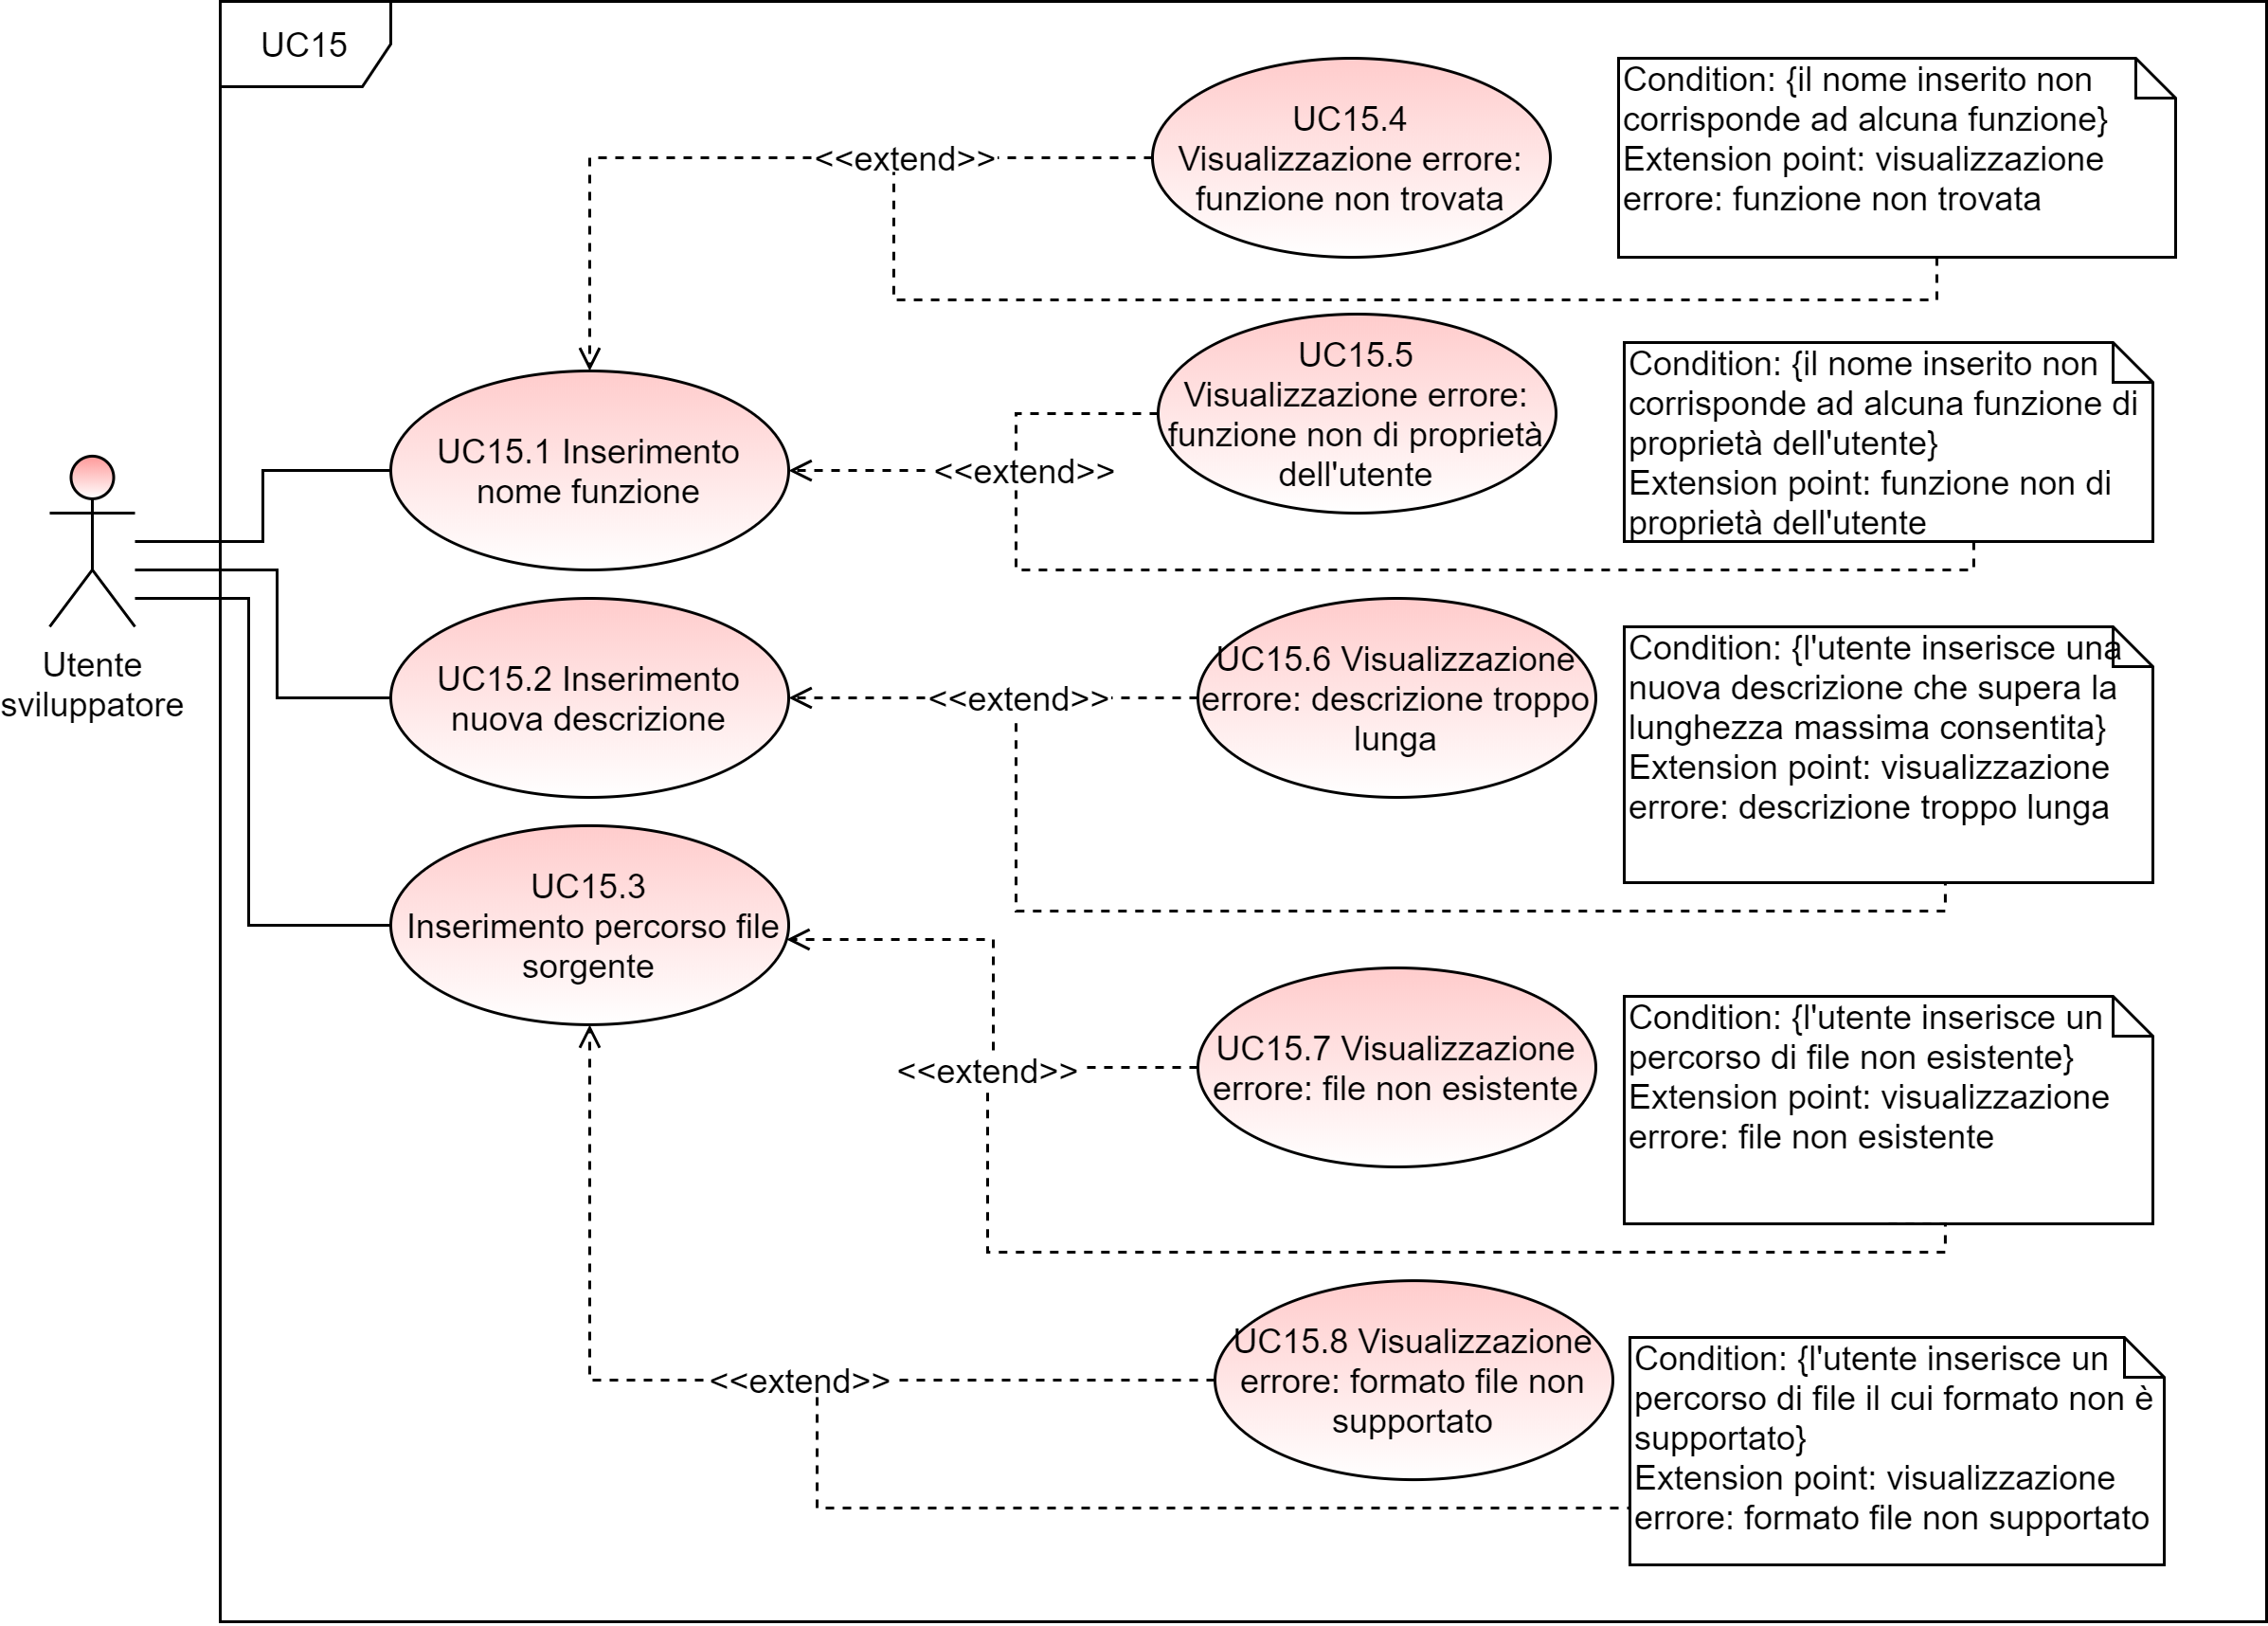
\includegraphics[scale=\ucs]{./res/img/UC15.png}
	\caption {UC15 - Modifica funzione }
\end{figure}
\begin{itemize}
	\item \textbf{Attori primari:} \us{};
	\item \textbf{Attori secondari:} \re{};
	\item \textbf{Descrizione:} l’utente richiede di modificare delle informazioni relative ad una sua funzione tramite il comando: \pedit{};
	\item \textbf{Scenario principale:} 
	\begin{itemize}
		\item  l’utente richiede la modifica di un’informazione relativa ad una propria funzione;
		\item il sistema modifica correttamente tale informazione.  
	\end{itemize}
	\item \textbf{Precondizione:} l’utente ha eseguito il deploy\ped{\textit{G}} di almeno una funzione
	\item \textbf{Postcondizione:} l’utente modifica correttamente la funzione. 
\end{itemize}